

%build with
%pdflatex main.tex 2>&/dev/null ; bibtex main 2>&/dev/null ; latexmk -pdf -f -g -bibtex -deps -synctex=1 -interaction=nonstopmode main.tex


%TC:macro \lstinline [xx]
%TC:envir lstlisting [] xall
\documentclass[12pt]{report}
\usepackage[paper=A4,pagesize]{typearea}
\usepackage{afterpage}
\usepackage[utf8]{inputenc}
\usepackage{graphicx}
\graphicspath{ {images/} }
\usepackage[hidelinks]{hyperref}
\usepackage[final]{pdfpages}
\usepackage{caption}
\usepackage{subcaption}
\usepackage[a4paper,width=175mm,top=25mm,bottom=25mm]{geometry}
\usepackage{fancyhdr}
\usepackage{enumitem}
\usepackage{float}
\usepackage{longtable}
\usepackage{amsmath}
\usepackage{xcolor}
\usepackage{amsmath}
\usepackage{array}
\usepackage{moreverb}
\usepackage{dirtree}
\usepackage{changepage}
\usepackage{tikz}
\usepackage[printonlyused,withpage]{acronym}
\pagestyle{fancy}
%puts chapter name in footer
\renewcommand{\chaptermark}[1]{\markboth{#1}{#1}}
\fancyhead{}
\fancyhead[R]{
Radiomics Approach to Diffusion MRI Tractography}
\fancyfoot{}
\fancyfoot[R]{\thepage}
\fancyfoot[L]{\leftmark}
\renewcommand{\headrulewidth}{0.4pt}
\renewcommand{\footrulewidth}{0.4pt}
\usepackage{titlesec}
%hides chapter text
\titleformat{\chapter}[display]{\normalfont\bfseries}{}{0pt}{\Huge}
\titlespacing*{\chapter}{0pt}{0pt}{30pt}
%paragraph indent
\setlength{\parindent}{12pt}
%paragraph spacing
\setlength{\parskip}{3pt}
%makes the numbering of the subsubsection alphabetical
\renewcommand{\thesubsubsection}{\thesubsection.\alph{subsubsection}}
\setcounter{secnumdepth}{4}
\setcounter{tocdepth}{2}
%creates left and right aligned table columns
\newcolumntype{R}[1]{>{\raggedleft\arraybackslash}p{#1}}
\newcolumntype{L}[1]{>{\raggedright\arraybackslash}p{#1}}
%code snippets
\usepackage{listings}
\usepackage{color}
\definecolor{dkgreen}{rgb}{0,0.6,0}
\definecolor{gray}{rgb}{0.5,0.5,0.5}
\definecolor{mauve}{rgb}{0.58,0,0.82}
\lstset{frame=tb,
  language=python,
  morekeywords={as},
  aboveskip=3mm,
  belowskip=3mm,
  showstringspaces=false,
  columns=fixed,
  basicstyle={\small\ttfamily},
  numbers=left,
  numberstyle=\tiny\color{gray},
  keywordstyle=\color{blue},
  commentstyle=\color{dkgreen},
  stringstyle=\color{mauve},
  breaklines=false,
  breakatwhitespace=true,
  tabsize=2
}
%references
\usepackage{csquotes}
\usepackage[utf8]{inputenc}
\usepackage[english]{babel}
\usepackage[backend=bibtex,sorting=none]{biblatex}
\addbibresource{references.bib}
%cite with clickable link wrapping some text as well
\newcommand{\citelink}[2]{\hyperlink{cite.\therefsection @#1}{#2} \cite{#1}}
%cite with clickable link wrapping some text as well
\newcommand{\reflink}[2]{\hyperref[#1]{#2} \ref{#1}}
%pdf details
\hypersetup{
  pdftitle={Enhancing Brain Connectivity Mapping: A Radiomics Approach to Diffusion MRI Tractography},
  pdfauthor={Levente Zsolt Nagy},
  pdfsubject={Medical Imaging},
  pdfkeywords={dMRI,MRI,magnetic resonance imaging,tractography,brain connectivity,radiomics,medical imaging},
  pdfcreator={Levente Zsolt Nagy},
}
%no break longtable hline
\makeatletter
\def\nobreakhline{%
  \noalign{\ifnum0=`}\fi
    \penalty\@M
    \futurelet\@let@token\LT@@nobreakhline}
\def\LT@@nobreakhline{%
  \ifx\@let@token\hline
    \global\let\@gtempa\@gobble
    \gdef\LT@sep{\penalty\@M\vskip\doublerulesep}
  \else
    \global\let\@gtempa\@empty
    \gdef\LT@sep{\penalty\@M\vskip-\arrayrulewidth}
  \fi
  \ifnum0=`{\fi}%
  \multispan\LT@cols
     \unskip\leaders\hrule\@height\arrayrulewidth\hfill\cr
  \noalign{\LT@sep}%
  \multispan\LT@cols
     \unskip\leaders\hrule\@height\arrayrulewidth\hfill\cr
  \noalign{\penalty\@M}%
  \@gtempa}
\makeatother
%title and author and date
\title{Enhancing Brain Connectivity Mapping: A Radiomics Approach to Diffusion MRI Tractography}
\author{Levente Zsolt Nagy}
\date{2024-12-15}
%word count
\immediate\write18{
  echo "Number of Words: " > wc.tex &&
  texcount main.tex -sum -1 -merge >> wc.tex &&
  echo "\\\\Number of Characters: " >> wc.tex &&
  texcount main.tex -sum -1 -merge -char >> wc.tex
}
%actual doc
\begin{document}
%TC:ignore
\begin{titlepage}
    \begin{center}
        \begingroup
          \let\clearpage\relax

          
\includegraphics[width=1\textwidth]{banner.png}
          \vfill
          \LARGE
          \begin{center}
          \textbf{\MakeUppercase{Predicting Brain Connectivity Mapping Using Radiomics Features in Anatomical MRI}}
          \end{center}
          \vfill
          \large
          \textbf{\MakeUppercase{Levente Zsolt Nagy}}
          \vfill
          \normalsize
          \textbf{Thesis supervisor}\\
          \MakeUppercase{Alfredo Vellido Alcacena} (Department of Computer Science)\\
          \hfill\\
          \textbf{Thesis co-supervisor}\\
          \MakeUppercase{Estela Camara Mancha} (Hospital Universitari de Bellvitge)\\
          \hfill\\
          \textbf{Degree}\\
          Master's Degree in Artificial Intelligence\\
          \hfill\\\hfill\\
          \textbf{Master's thesis}\\
          \hfill\\
          \textbf{School of Engineering}\\
          \textbf{Universitat Rovira i Virgili (URV)}\\
          \hfill\\
          \textbf{Faculty of Mathematics}\\
          \textbf{Universitat de Barcelona (UB)}\\
          \hfill\\
          \textbf{Barcelona School of Informatics (FIB)}\\
          \textbf{Universitat Politècnica de Catalunya (UPC) - BarcelonaTech}\\
%           \Huge
%           \textbf{Enhancing Brain Connectivity Mapping:\\
%             A Radiomics Approach to\\
%             Diffusion MRI Tractography}

%           \vspace{0.1cm}
%           \LARGE
%           Medical Imaging

%           \vspace{1.0cm}

%           Levente Zsolt Nagy\\
%           \vspace{1.0cm}
%           \Large
%           \emph{Supervisors}\\
%           Estela Camara Mancha\\
%           Alfredo Vellido Alcacena\\
%           \LARGE

%           \vfill

%           A thesis presented for the degree of\\
%           Master in Artificial Intelligence

%           \vspace{1.0cm}
%           \includegraphics[width=0.37\textwidth]{upc.png}\\
%           \vspace{0.2cm}
%           \hspace{7px}\includegraphics[width=0.37\textwidth]{ub.png}\\
%           \vspace{0.2cm}
%           \includegraphics[width=0.37\textwidth]{bellvitge.png}\\
%           \vspace{1.0cm}

%           \Large
%           Universitat Politècnica de Catalunya\\
%           Universitat de Barcelona\\
%           Hospital Universitari de Bellvitge\\
%           Spain\\
%           2024-12-15\\
%           Number of Words: 
681
\\Number of Characters: 
3682


        \endgroup
    \end{center}
\end{titlepage}
%TC:endignore
\thispagestyle{plain}
\begin{center}
    \Large
    \textbf{Abstract}
\end{center}
\textit{Anatomical magnetic resonance imaging (MRI), such as T1 and T2 weighted images, are commonly used to distinguish brain tissue types. Diffusion tensor imaging (DTI), a more specialized MRI technique, enables the mapping of white matter and the study of structural connectivity through metrics like fractional anisotropy (FA) and mean diffusivity (MD). However, DTI acquisition is time intensive and often excluded from standard clinical protocols.}\par
\textit{This study introduces a method to synthesize FA and MD images from widely available T1 and T2 weighted anatomical scans, reducing dependence on resource intensive DTI acquisition.}\par
\textit{Radiomics, a rapidly evolving field, focuses on extracting quantitative features from medical imaging, to identify biomarkers associated with clinical labels. It is a well established tool in oncology, particularly for tumor segmentation. Fully convolutional neural networks (FCNNs) are also employed for similar tasks, such as deriving clinical labels for tumor segmentation. However, their reliance on computationally intensive 3D convolutions often necessitates the use of 2D slices from 3D volumes, limiting their feasibility.}\par
\textit{We present a hybrid approach that combines the strengths of radiomics and neural networks. Specifically, we use a feedforward neural network (FNN) as a classification or regression head applied to radiomic features, preserving 3D spatial information during feature extraction while reducing the computational demands of 3D convolutions. This neural network head, akin to fully connected layers in traditional convolutional neural networks (CNNs), offers significant flexibility.}\par
\textit{Our experiments are limited to the basal ganglia, a crucial region involved in brain structure and function that is significantly impacted by neurodegeneration in Huntington’s disease (HD). The inclusion of HD patients allows for assessing the method's reliability and robustness. Additionally, we explore the potential of using the T1/T2 ratio as an input image, which has been proposed in recent studies, as a proxy for the myelin content of the brain. Since myelin plays a role in how DTI functions, the T1/T2 ratio may enhance model performance, effectively bridging anatomical MRI and DTI.}\par
\textit{The results indicate strong performance, with Pearson correlations of 85\% for FA and 95\% for MD predictions. While the correlation decreases significantly for FA and moderately for MD in HD patients, the model’s performance remains consistent when both healthy controls and patients are analyzed together. These findings underscore the promise of our hybrid approach for synthesizing structural connectivity images and improving accessibility to diffusion metrics.}
%TC:ignore
\tableofcontents
\chapter*{List of Notations \& Abbreviations}
\begin{acronym}\itemsep0pt
  \acro{MRI}{magnetic resonance imaging}
  \acro{dMRI}{diffusion magnetic resonance imaging}
  \acro{ROI}{region of interest}
  \acro{FNN}{fully connected neural network}
  \acro{FCNN}{fully convolutional neural network}
  \acro{NIfTI}{Neuroimaging Informatics Technology Initiative}
  \acro{GLCM}{Gray Level Co-occurrence Matrix}
  \acro{GLSZM}{Gray Level Size Zone Matrix}
  \acro{GLRLM}{Gray Level Run Length Matrix}
  \acro{NGTDM}{Neighbouring Gray Tone Difference Matrix}
  \acro{GLDM}{Gray Level Dependence Matrix}
\end{acronym}
\listoffigures
\listoftables
%TC:endignore

\chapter{Introduction}
\citelink{basal}{Basal ganglia is a part of the human brain which is group of subcortical nuclei responsible primarily for motor control, as well as other roles such as motor learning, executive functions and behaviors, and emotions.} \citelink{hunting}{Huntington’s disease is a disorder that causes the progressive degeneration of the basal nuclei.}\par

Hospital de Bellvitge provided an excellent dataset of \ac{MRI} and \ac{dMRI} records. This dataset contains 32 control and 37 Huntington patient records of T1 and T1/T2 \ac{MRI} images with isotropic voxels of 1 millimeter resolution and \ac{dMRI} \ac{FA}, \ac{MD} and \ac{RD} images with isotropic voxels of 2 millimeter resolution and 1 second temporal resolution. Furthermore this dataset also contains the mask for the basal ganglia, which will also be referenced as the \ac{ROI}. And taking inspiration from this \citelink{conn}{paper}, masks for the 7 main cortical regions of the brain, which will also be referenced as the target regions: Limbic, Executive, Rostral-Motor, Caudal-Motor, Parietal, Occipital and Temporal are also included in the dataset. Tractography was performed on the \ac{dMRI} images to figure out which parts of the \ac{ROI} are connected to which cortical target, in a similar manner to how it was done in said \citelink{conn}{paper}; where the relative connectivity maps are representing the ratio of the number of streamlines to each cortical target. Furthermore, the raw streamline images are also available, where there are a maximum of 5000 streamlines from each voxel in the \ac{ROI}. The anatomical segmentation of the Basal Ganglia is also available, for the Caudate Putamen and Accumbens. \par

\begin{figure}[H]
\centering
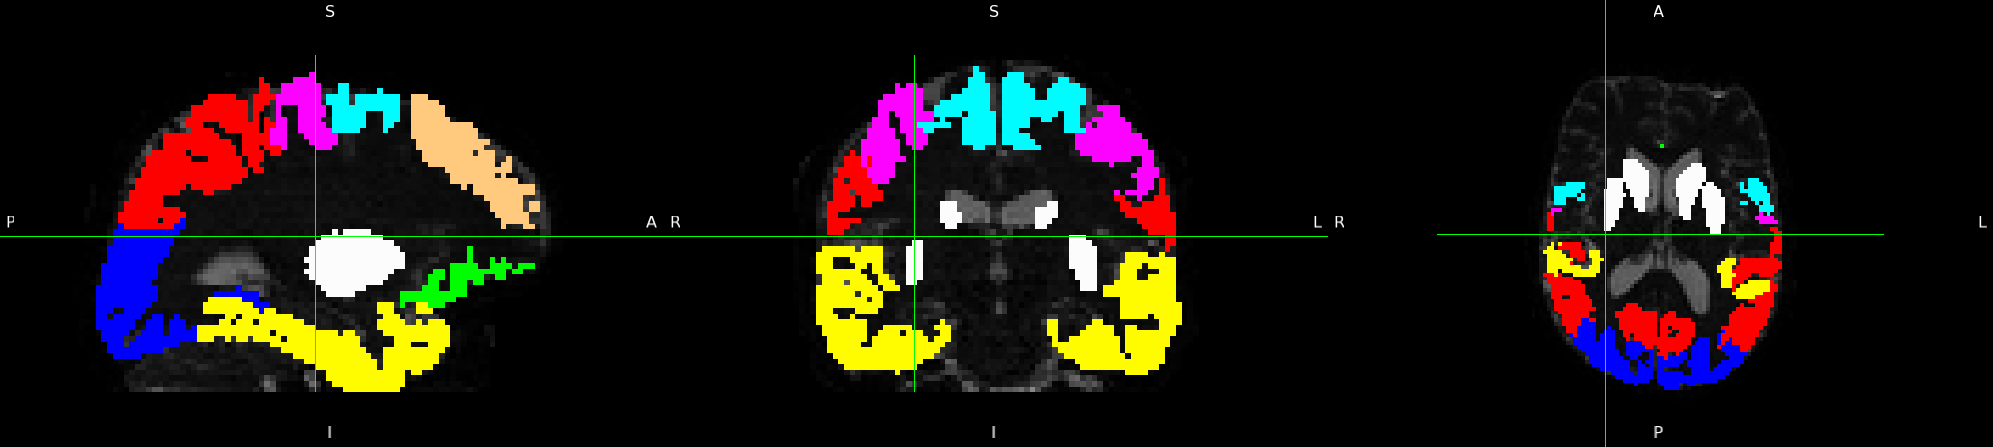
\includegraphics[width=1\textwidth]{rois}
\caption{Basal Ganglia (ROI) \& Cortical Targets}
\label{fig:rois}
\end{figure}

\begin{table}[H]
\centering
\begin{tabular}{|l|l|}
\hline
\textbf{Color} & \textbf{Region} \\ \hline
\begin{tikzpicture}\filldraw[draw=black,fill={rgb,255:red,255;green,255;blue,255}](0,0.15)rectangle(0.25,0.4);\end{tikzpicture} White & Basal Ganglia (ROI) \\ \hline

\begin{tikzpicture}\filldraw[draw=black,fill={rgb,255:red,0;green,255;blue,15}](0,0.15)rectangle(0.25,0.4);\end{tikzpicture} Green & Limbic \\ \hline
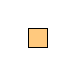
\begin{tikzpicture}\filldraw[draw=black,fill={rgb,255:red,255;green,201;blue,126}](0,0.15)rectangle(0.25,0.4);\end{tikzpicture} Brown & Executive \\ \hline

\begin{tikzpicture}\filldraw[draw=black,fill={rgb,255:red,0;green,252;blue,255}](0,0.15)rectangle(0.25,0.4);\end{tikzpicture} Light Blue & Rostral-Motor \\ \hline
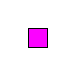
\begin{tikzpicture}\filldraw[draw=black,fill={rgb,255:red,251;green,3;blue,255}](0,0.15)rectangle(0.25,0.4);\end{tikzpicture} Purple & Caudal-Motor \\ \hline
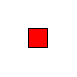
\begin{tikzpicture}\filldraw[draw=black,fill={rgb,255:red,253;green,0;blue,0}](0,0.15)rectangle(0.25,0.4);\end{tikzpicture} Red & Parietal \\ \hline

\begin{tikzpicture}\filldraw[draw=black,fill={rgb,255:red,0;green,0;blue,253}](0,0.15)rectangle(0.25,0.4);\end{tikzpicture} Blue & Occipital \\ \hline

\begin{tikzpicture}\filldraw[draw=black,fill={rgb,255:red,255;green,252;blue,0}](0,0.15)rectangle(0.25,0.4);\end{tikzpicture} Yellow & Temporal \\ \hline
\end{tabular}
\caption{Regions Legend}
\label{tab:reglen}
\end{table}

Furthermore, for both the \ac{ROI} and cortical targets, the dataset distinguishes between the right and left halves of the brain. Thus there are actually 2 \ac{ROI}s and $2 \cdot 7=14$ target regions.

\begin{figure}[H]
\centering
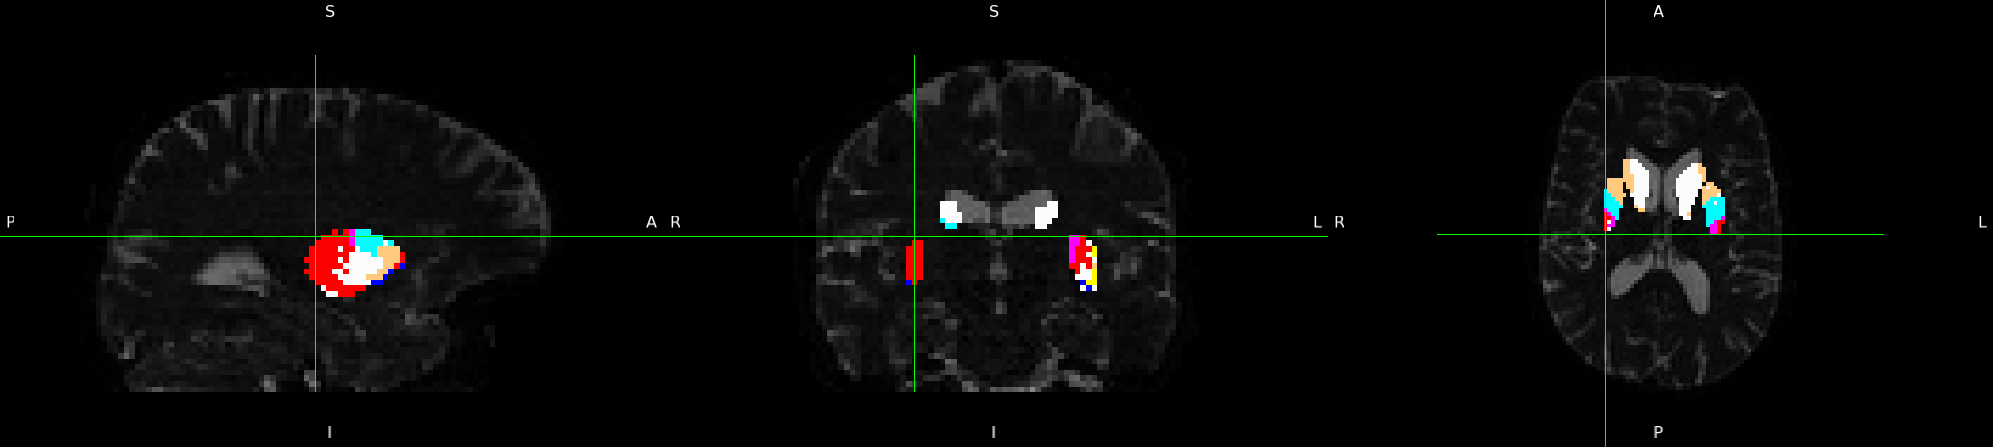
\includegraphics[width=1\textwidth]{conn}
\caption{Connectivity Maps}
\label{fig:conn}
\end{figure}

\section{Objectives}

The end goal is to predict the relative connectivity of the Basal Ganglia to the cortical targets, from the T1 and T1/T2 images.\par

This being a very complex problem, there is the possibility that the correlation between the connectivity of the brain and the T1, T1/T2 images are too weak to be mapped on this dataset. As from a datascience perspective, 69 datapoints are not much. But from a medical perspective it is substantial as it is very hard to collect uniform, clean data, with permissions to use it for research.\par

As a simpler task, leading up to the complex end goal, is a model for the simple segmentation of the Basal Ganglia for the regions Caudate Putamen and Accumbens. In order to confirm that the radiomics texture of the T1 and T1/T2 images of this dataset are are correlated to the anatomical segmentation of the Basal Ganglia. This problem is inherently connected to the main goal, as the relative connectivity does obey certain anatomical restrictions, and the anatomical segmentation of the Basal Ganglia is confirmed to be related to the relative connectivity. Thus if this simpler prediction fails, there is a good chance that the complex end goal will fail as well.\par

The biggest obstacle of this project is the preprocessing of the data, as there are many variations and hyperparameters that can be tuned. An exhaustive search definetly will not be viable, thus the preprocessing and model will needed to be tuned in a waterfall like manner, making educated guesses and comparing model performances across different tries. The main metric to measure model performance, will be the accuracy of the label prediction across voxels, as it should be comparable between all approaches.

\section{Motivation}

The motivation for predicting the connectivity maps from the T1 and T1/T2 \ac{MRI} images, is skipping the time and resource consuming process performing \ac{dMRI} and tractorgrapy.

\section{State of the Art}

Me :)




























\chapter{Requirements}
The following requirements were defined based on the objectives of this thesis:

\begin{enumerate}
  \item Preprocess the data.
  \item Extract radiomics features.
  \item Observe direct correlations between extracted features and connectivity maps.
  \item Design a decision tree for predicting the connectivity maps from the extracted features.
  \item Design an \ac{FNN} for predicting the connectivity maps from the extracted features.
  \item Grid search radiomics feature extraction parameters for the best results.
  \item Design an \ac{FCNN} for predicting the connectivity maps from the T1 image.
  \item Modify the \ac{FCNN} by appending the \ac{ROI} mask to the input.
  \item Modify the \ac{FCNN} by appending the cortical target masks to the input.
  \item Design a generalized \ac{FCNN} for predicting one connectivity map at a time from the T1 image, \ac{ROI} \& target masks.
\end{enumerate}

\chapter{Preprocessing}
\section{Raw Data}
All provided data are in the \ac{NIfTI} format, first these are need to be understood and parsed. This format stores the raw output of the \ac{MRI} record, and additionally a transformation matrix which can translate this raw space into anatomical space. The process of aligning different records into the same anatomical space is called "registration". The provided dataset's T1 \ac{MRI} and \ac{dMRI} records are already registered in the same space.

\subsection{Available Data}
The following data will be preprocessed and read, even if not all of them are going to be used later on it helps providing the largest possible flexibility later on.
\begin{table}[H]
\centering
\begin{tabular}{|l|l|c|c|l|l|}
\hline
\textbf{Data} & \textbf{Shape} & \textbf{Range} & \textbf{Type} & \textbf{Space} & \textbf{Reference} \\ \hline
\ac{dMRI} & (118, 118, 60, 74) & $[0,2492]$ & float16 & diffusion & diffusion \\ \hline
T1 & (208, 256, 256) & $[0,629]$ & float16 & t1 & t1 \\ \hline
\ac{ROI} Mask (Basal Ganglia) & (118, 118, 60) & $\{0,1\}$ & bool & diffusion & roi \\ \hline
Cortical Targets & (118, 118, 60, 7) & $\{0,1\}$ & bool & diffusion & targets \\ \hline
Relative Connectivity & (118, 118, 60, 7) & $[0,1]$ & float16 & diffusion & connectivity \\ \hline
\ac{dMRI} Brain Mask & (118, 118, 60) & $\{0,1\}$ & bool & diffusion & diffusion\_mask \\ \hline
T1 Brain Mask & (208, 256, 256) & $\{0,1\}$ & bool & t1 & t1\_mask \\ \hline
\end{tabular}
\caption{Raw Datapoint}
\label{tab:datas1}
\end{table}

\subsection{Brain Mask}
The provided dataset did not apply the brain masks out of the box so it can be done with a simple element wise multiplication.

\subsection{Anatomical Space}
Transforming two different readings into the same anatomical space still requires a bit of math. As after applying the extracted transformation matrices, the records will line up, but the center of the voxel space will be at $(0,0,0)$. Meaning that technically only the first quadrant will be visible of the record, thus the space is also needed to be translated with the negative vector of the transformed space's bounding box's lower end.\par
The translation value can be calculated by calculating the boundaries of the transformed space's bounding box. Get all 8 corners of the voxel space and apply the transformation matrix to all of them. Then get the min-max coordinates along X, Y and Z from the 8 transformed vectors, yielding the lower and upper bounds of the transformed space's bounding box.\par
It is very important to use the same translation value across different raw spaces to properly align them in the anatomical space. For example let $D$ and $T$ denote a diffusion and t1 records and $M_D$ and $M_T$ denote their respective transformation matrices. Let $T_D$ and $T_T$ denote their respective translation values. In order to properly align them we need to apply $A_D = (M_D \cdot {\color{red}T_D})$ matrix and $A_T = (M_T \cdot {\color{red}T_D})$ matrix to $D$ and $T$ respectively, with matching ${\color{red}T_D}$ translation values.\par
The last issue is the missaligned new shapes of the T1 and Diffusion records. This can be simply fixed by truncating the excess along each dimension.

\subsection{Uniform Shape}
After aligning the data into the same space per datapoint, it is still very likely that the individual datapoints do not have a uniform shape. This is due to them being registered into the same space datapoint wise, but can have differrent registrations across multiple datapoints.\par
Fixing this can be done by figuring out the min-max boundaries along each axis that the brain masks take up in the voxel space. Then the range of the masks along each axis can be calculated from the lower and upper boundaries per datapoint. And then the max range can be selected per axis, across all datapoints, yielding the new uniform shape. Finally, the voxel spaced can be sliced down to the new uniform shape, which can fit all brain masks of all data points.\par
Note that this fix also greatly improves space efficiency, as it cuts out the unused voxels. This will be beneficial for storage and computational demands of future experiments.
\begin{table}[H]
\centering
\begin{tabular}{|l|l|c|c|}
\hline
\textbf{Data} & \textbf{Shape} & \textbf{Range} & \textbf{Type} \\ \hline
diffusion & (80, 150, 186, 124, 74) & $[0,2492]$ & float16 \\ \hline
t1 & (80, 150, 186, 124, 1) & $[0,629]$ & float16 \\ \hline
roi & (80, 150, 186, 124, 1) & $\{0,1\}$ & bool \\ \hline
targets & (80, 150, 186, 124, 7) & $\{0,1\}$ & bool \\ \hline
connectivity & (80, 150, 186, 124, 7) & $[0,1]$ & float16 \\ \hline
diffusion\_mask & (80, 150, 186, 124, 1) & $\{0,1\}$ & bool \\ \hline
t1\_mask & (80, 150, 186, 124, 1) & $\{0,1\}$ & bool \\ \hline
\end{tabular}
\caption{Uniform Data}
\label{tab:datas2}
\end{table}
Note that the new shapes are all 5 dimensional, where the first dim is for the datapoint index. The next 3 is for the coordinates of the voxel space. And the last is for any additional information, like the temporal dimension of the \ac{dMRI} or the target masks or the connectivity labels.

\section{Radiomics Features}
Extracting the voxel based radiomic features has two main parameters to tune, the bin width and the kernel width.\par
The two main approaches for binning are absolute discretization and relative discretization. Where in the prior one, a fixed bin width is choosen and in the latter one, a fixed number of bins are chosen and the bin width scales relatively according to the min-max voxel values. \citelink{bin}{This study found that "The absolute discretization consistently provided statistically significantly more reproducible features than the relative discretization."} Relying on this information, the obvious choice is the absolute discretization.\par
The bin width and the kernel width will be tuned in later experiments. And possibly features calculated with different setting will be concatenated and used simultaneously for better results. The used default values will be 25 and 5 for the bin and kernel widths respectively.\par
The following types of radiomic features will be used:
\begin{table}[H]
\centering
\begin{tabular}{|l|c|}
\hline
\textbf{Feature Type} & \textbf{Number of Features} \\ \hline
First Order & 18 \\ \hline
\ac{GLCM} & 23 \\ \hline
\ac{GLSZM} & 16 \\ \hline
\ac{GLRLM} & 16 \\ \hline
\ac{NGTDM} & 5 \\ \hline
\ac{GLDM} & 14 \\ \hline
3D Shape & 17 \\ \hline
\end{tabular}
\caption{Radiomic Feature Types}
\label{tab:radf0}
\end{table}

\subsection{Voxel Based}
The following 92 features will be calculated voxel based:
\bgroup
\setlength\LTleft{-1cm}
\setlength\LTright{-1cm}
\begin{longtable}[H]{|l|l|l|}
\nobreakhline
\textbf{First Order} & \textbf{\ac{GLCM}} & \textbf{\ac{GLSZM}} \\ \nobreakhline
Energy & Autocorrelation & SmallAreaEmphasis \\ \nobreakhline
TotalEnergy & JointAverage & LargeAreaEmphasis \\ \nobreakhline
Entropy & ClusterProminence & GrayLevelNonUniformity \\ \nobreakhline
Minimum & ClusterShade & GrayLevelNonUniformityNormalized \\ \nobreakhline
10Percentile & ClusterTendency & SizeZoneNonUniformity \\ \nobreakhline
90Percentile & Contrast & SizeZoneNonUniformityNormalized \\ \nobreakhline
Maximum & Correlation & ZonePercentage \\ \nobreakhline
Mean & DifferenceAverage & GrayLevelVariance \\ \nobreakhline
Median & DifferenceEntropy & ZoneVariance \\ \nobreakhline
InterquartileRange & DifferenceVariance & ZoneEntropy \\ \nobreakhline
Range & JointEnergy & LowGrayLevelZoneEmphasis \\ \nobreakhline
MeanAbsoluteDeviation & JointEntropy & HighGrayLevelZoneEmphasis \\ \nobreakhline
RobustMeanAbsoluteDeviation & Imc1 & SmallAreaLowGrayLevelEmphasis \\ \nobreakhline
RootMeanSquared & Imc2 & SmallAreaHighGrayLevelEmphasis \\ \hline
Skewness & Idm & LargeAreaLowGrayLevelEmphasis \\ \nobreakhline
Kurtosis & MCC & LargeAreaHighGrayLevelEmphasis \\ \nobreakhline
Variance & Idmn &  \\ \nobreakhline
Uniformity & Id &  \\ \nobreakhline
 & Idn &  \\ \nobreakhline
 & InverseVariance &  \\ \nobreakhline
 & MaximumProbability &  \\ \nobreakhline
 & SumEntropy &  \\ \nobreakhline
 & SumSquares &  \\ \hline \hline
\textbf{\ac{GLRLM}} & \textbf{\ac{NGTDM}} & \textbf{\ac{GLDM}} \\ \nobreakhline
ShortRunEmphasis & Coarseness & SmallDependenceEmphasis \\ \nobreakhline
LongRunEmphasis & Contrast & LargeDependenceEmphasis \\ \nobreakhline
GrayLevelNonUniformity & Busyness & GrayLevelNonUniformity \\ \nobreakhline
GrayLevelNonUniformityNormalized & Complexity & DependenceNonUniformity \\ \nobreakhline
RunLengthNonUniformity & Strength & DependenceNonUniformityNormalized \\ \nobreakhline
RunLengthNonUniformityNormalized &  & GrayLevelVariance \\ \nobreakhline
RunPercentage &  & DependenceVariance \\ \nobreakhline
GrayLevelVariance &  & DependenceEntropy \\ \nobreakhline
RunVariance &  & LowGrayLevelEmphasis \\ \nobreakhline
RunEntropy &  & HighGrayLevelEmphasis \\ \nobreakhline
LowGrayLevelRunEmphasis &  & SmallDependenceLowGrayLevelEmphasis \\ \nobreakhline
HighGrayLevelRunEmphasis &  & SmallDependenceHighGrayLevelEmphasis \\ \nobreakhline
ShortRunLowGrayLevelEmphasis &  & LargeDependenceLowGrayLevelEmphasis \\ \nobreakhline
ShortRunHighGrayLevelEmphasis &  & LargeDependenceHighGrayLevelEmphasis \\ \nobreakhline
LongRunLowGrayLevelEmphasis &  &  \\ \nobreakhline
LongRunHighGrayLevelEmphasis &  &  \\ \nobreakhline
\caption{Voxel Based Radiomic Features}
\label{tab:radf1}
\end{longtable}
\egroup

\subsubsection{Normalization}


\subsection{Non-Voxel Based}
ASFD







\chapter{Models}
\input{chapters/models}
\chapter{Results}
\input{chapters/results}
\chapter{Implementation}
\label{implementation}
\chapter{Conclusions}
\label{sec:conclusions}

This foundational project has huge potential thanks to the possible return and applications of the used approach. Due time and resource limitations, the experiments only focused on the Basal Ganglia, so by no means any of the performance metrics prove that a generalized solution is viable. However the \ac{FA} and \ac{MD} predictions are really promising, and would be interesting to see how would it perform on the entire brain, and not just the \ac{ROI}. On the other hand the Relative Connectivity predictions are not even nearly precise enough to call them usable, but admittedly the labels themselves will inherently contains quite a bit of noise, due to the very sensitive process extracting the labels with tractography.\par
This project only delved into a tiny fraction of the endless sea of possible preprocessing approaches, and it only experimented with some very basic model architectures. Nevertheless, the viability of this approach and hypothesis is not disproven, but it definitely needs some new ideas implemented to make it work.\par

\section{Future Improvements}
\label{sec:improve}

As mentioned in \reflink{sec:seqback}{subsection}, there was a serious oversight during the execution of the exhaustive sequential backwards feature selection. At the time it was believed that the model was performing better on balanced data, due to a bug in the code. Thus, all of these models are performing much worse than the models during the experimentation. The bug was fixed, but due to limited time and resources the feature selection was not executed again.\par
Further investigating the sex imbalance issue discovered in \reflink{sec:inclusive}{subsection}, reveals that with the used seed for the experimentation is not terribly imbalanced for the most part, but there are definitely room for improvement by enforcing a constant ratio. The male/(male+female) ratio for the control record splits are $0.49$/$0.67$/$0.67$ (train/validation/test), and for the patient records are $0.62$/$0.5$/$1$.\par
Besides these known mistakes, there are some issues that are hard to quantify. For example due to the different imaging of the anatomical records and the \ac{DTI} record, even after a perfect affine registration they can have tiny misalignments. Explained by the records being taken separately, possible physiological movements, and independent preprocessing steps. This may be the reason behind the normalized experiments performing better than the native experiments in most cases, as the normalized images have less discrepancy between them.\par
Additionally, one aspect was not investigated thoroughly during this project and that being the kernel size, binning parameters, and feature class relationships, during the voxel based feature extraction. For the sake of simplicity, only a unified binning method was used for all kernel sizes and all feature classes. But logically the binning parameters could be optimized for each kernel size and feature class. For example logically the \ac{GLRLM} feature class could yield fundamentally different features even just by adjusting the bin size a tiny bit at large kernel sizes.\par
Selecting the most efficient kernel size combinations were not investigated thoroughly either. Due to limited resources, the maximum kernel size used was 21, but there were no reason to stop here (besides to be able to finish this project in time).\par
Ultimately, even with the 'few' simple aspects that were taken into consideration during this project, the hyperparameter space is gigantic and some compromises were had to be made. After investing over 500 hours into this project, the educated guesses for these potential improvements are:
\begin{itemize}
  \item The feature selection should have a marginal improvement on the model performance.
  \item The gender imbalance should not have a measurable impact on the model performance on this scale (with less than 70 available records in total).
  \item The binning parameter optimization for the kernel sizes and feature classes would probably have a big impact on the model performance.
\end{itemize}
And lastly, all experiments should be repeated at least a few times, with different splits and seeds. And the experiments should be evaluated with the means and medians of the model performance indicators, across different runs.

\section{Project Future}

Ultimately there are two paths to continue this project. First, the \ac{FA} and \ac{MD} experiments could be expanded to the entire brain and a generalized model should be developed. And the other being the refinement of the Relative Connectivity experiments, as it definitely need improvements and new ideas.



\chapter{Future Imporvements}
\input{chapters/future}

%TC:ignore
\printbibliography[heading=bibintoc,title={Sources of Information}]
\appendix

%================== EXAMPLES ==================
% \includepdf[pages=1,pagecommand={\chapter[Project Description]{} \label{app:projdesc}},linktodoc=true]{Appendix_A/ProjectDescription.pdf}
% \includepdf[pages=2-]{Appendix_A/ProjectDescription.pdf}
% \chapter{Machine Vision Class Descriptions} \label{app:CVclassdesc}
% \input{appendices/classdesccpp}
% \chapter{Source Code} \label{app:sourcecode}
% \label{apx:source}

\dirtree{%
.1 source.
.2 data.
.3 models.
.3 native.
.4 preloaded.
.4 preprocessed.
.4 raw.
.3 normalized.
.4 preloaded.
.4 preprocessed.
.4 raw.
.3 preprocessed.
.3 raw.
.2 logs.
.2 fsleyes.
.2 distributed.
.1 experiments.
.2 subcortical.
.2 diffusion\_md.
.3 native-t1.
.3 native-t1t2.
.3 normalized-t1.
.3 normalized-t1t2.
.3 architecture.
.2 diffusion\_fa.
.3 native-t1.
.3 native-t1t2.
.3 normalized-t1.
.3 normalized-t1t2.
.3 architecture.
.2 connection.
.3 native-t1.
.3 native-t1t2.
.3 normalized-t1.
.3 normalized-t1t2.
.3 architecture.
.2 streamline.
.2 misc.
.1 report.
.2 progress.
.2 project.
}


% \texttt{ }\par
% \noindent \textbf{android-camera-imu} the source code of the auxiliary camera-imu app\par
% \texttt{ }\par
% \noindent \textbf{diagrams} exported UML diagrams\par
% \texttt{ }\par
% \noindent \textbf{doc} some of the \path{.tex} files\par
% \noindent \textbf{appendices} appendix \path{.tex} files\par
% \noindent \textbf{chapters} chapter \path{.tex} files\par
% \noindent \textbf{images} figures\par
% \includepdf[pages=1,pagecommand={\chapter[User Manual]{} \label{app:manual}},linktodoc=true]{Appendix_D/UserManual.pdf}
% \includepdf[pages=2-]{Appendix_D/UserManual.pdf}
% \chapter{Unit Test Descriptions and Test Results} \label{app:CVunittestdesc}
% \input{appendices/unittestdesccpp}
% \chapter{Integration Test Results} \label{app:CVintegrationtestdesc}
% \input{appendices/integrationtestdesccpp}
% \includepdf[pages=1,pagecommand={\chapter[Process Report]{} \label{app:procrep}},linktodoc=true]{Appendix_G/ProcessReport.pdf}
% \includepdf[pages=2-]{Appendix_G/ProcessReport.pdf}
%==============================================

%TC:endignore
\end{document}